\documentclass[border=2pt]{standalone}
\usepackage{amssymb}
\usepackage{amsmath}
\usepackage{array}
\usepackage{colortbl}
\usepackage{tikz}
\usetikzlibrary{positioning, shapes.geometric}

\definecolor{cnavy}{HTML}{0E2747}
\definecolor{corange}{HTML}{E8573F}
\definecolor{cgreen}{HTML}{3B9B6D}
\definecolor{cslate}{HTML}{5B6680}
\definecolor{cmuted}{HTML}{9B9484}
\definecolor{ccream}{HTML}{FAFAF6}
\definecolor{cwarn}{HTML}{D08D2A}

\definecolor{rowA}{HTML}{F4F7FA}
\definecolor{rowB}{HTML}{FAFAF6}
\definecolor{headerBg}{HTML}{0E2747}

\newcommand{\yesmark}{\textcolor{cgreen}{\textbf{yes}}}
\newcommand{\nomark}{\textcolor{corange}{\textbf{no}}}
\newcommand{\openmark}{\textcolor{cwarn}{\textbf{research}}}

\begin{document}
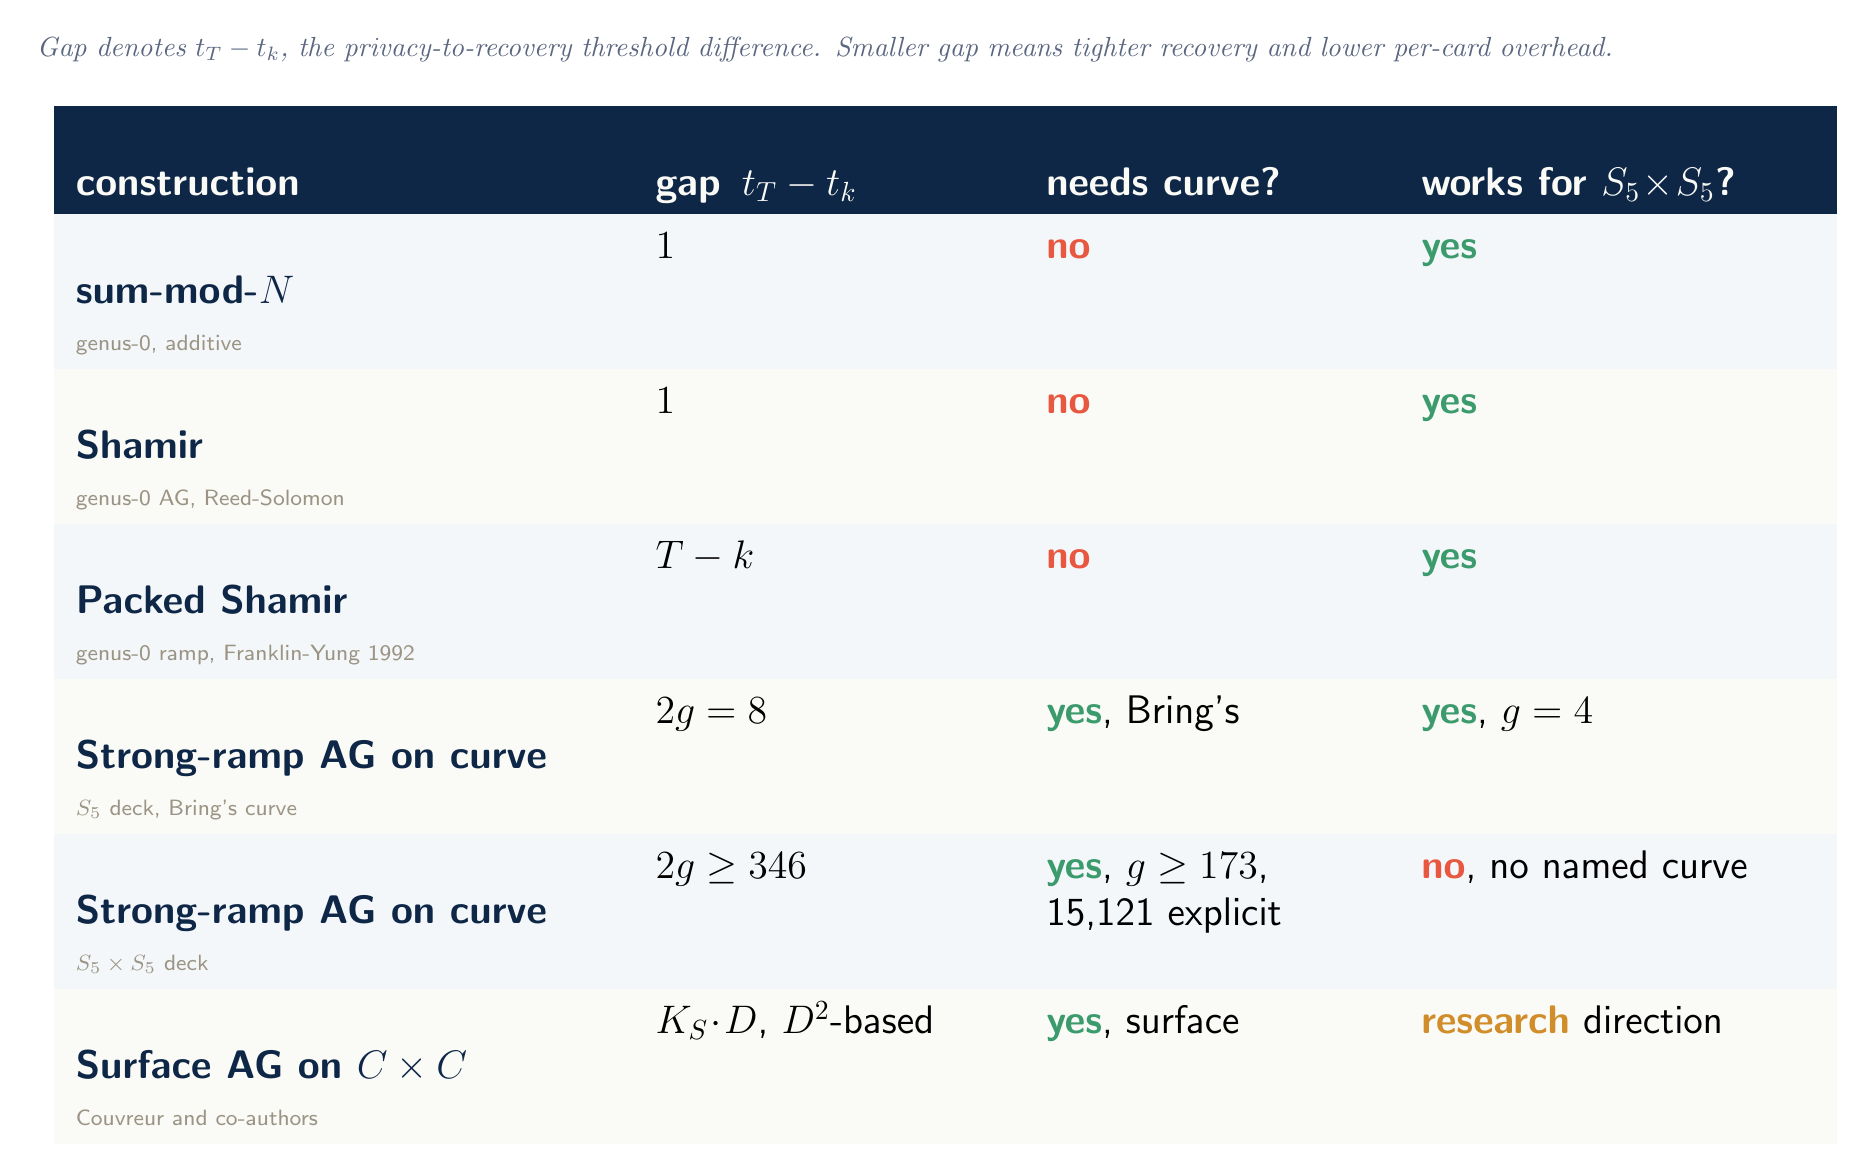
\begin{tikzpicture}[font=\sffamily]

\node[cslate, font=\itshape\normalsize, anchor=north west, text width=22cm]
  at (0, 0)
  {Gap denotes $t_T - t_k$, the privacy-to-recovery threshold difference.
   Smaller gap means tighter recovery and lower per-card overhead.};

\node[anchor=north west, inner sep=0pt] at (0, -1.0) {%
\fontsize{14pt}{17pt}\selectfont
\renewcommand{\arraystretch}{1.35}
\setlength{\tabcolsep}{8pt}
\begin{tabular}{
  >{\raggedright\arraybackslash}p{6.8cm}
  >{\raggedright\arraybackslash}p{4.4cm}
  >{\raggedright\arraybackslash}p{4.2cm}
  >{\raggedright\arraybackslash}p{5.0cm}
}
\rowcolor{headerBg}
{\color{ccream}\bfseries construction} &
{\color{ccream}\bfseries gap $\,t_T - t_k$} &
{\color{ccream}\bfseries needs curve?} &
{\color{ccream}\bfseries works for $S_5 \!\times\! S_5$?} \\
\rowcolor{rowA}
{\color{cnavy}\bfseries sum-mod-$N$}\newline
{\color{cmuted}\footnotesize genus-0, additive}
 & $1$
 & \nomark
 & \yesmark \\
\rowcolor{rowB}
{\color{cnavy}\bfseries Shamir}\newline
{\color{cmuted}\footnotesize genus-0 AG, Reed-Solomon}
 & $1$
 & \nomark
 & \yesmark \\
\rowcolor{rowA}
{\color{cnavy}\bfseries Packed Shamir}\newline
{\color{cmuted}\footnotesize genus-0 ramp, Franklin-Yung 1992}
 & $T - k$
 & \nomark
 & \yesmark \\
\rowcolor{rowB}
{\color{cnavy}\bfseries Strong-ramp AG on curve}\newline
{\color{cmuted}\footnotesize $S_5$ deck, Bring's curve}
 & $2g = 8$
 & \yesmark, Bring's
 & \yesmark, $g = 4$ \\
\rowcolor{rowA}
{\color{cnavy}\bfseries Strong-ramp AG on curve}\newline
{\color{cmuted}\footnotesize $S_5 \times S_5$ deck}
 & $2g \geq 346$
 & \yesmark, $g \geq 173$,\newline 15{,}121 explicit
 & \nomark, no named curve \\
\rowcolor{rowB}
{\color{cnavy}\bfseries Surface AG on $C \times C$}\newline
{\color{cmuted}\footnotesize Couvreur and co-authors}
 & $K_S \!\cdot\! D$, $D^2$-based
 & \yesmark, surface
 & \openmark{} direction \\
\end{tabular}%
};

\end{tikzpicture}
\end{document}
